% Map-reduce summarization pipeline (Stage 2) — schematic for the paper.
% One hearing transcript -> turn-boundary chunks -> map (one call per chunk)
% -> token-budget check -> conditional collapse rounds -> reduce -> final
% summary sized to the sentence-encoder window. All numbers are measured on
% the SST corpus (2,352 hearings); constants from lib/summarize.py
% (prompt hearing-mapreduce-1.0) and 03_summarize_sst (CHUNK_TOKENS=6144).
% Compile: xelatex fig_summarization_mapreduce.tex
\documentclass[tikz]{standalone}
\usetikzlibrary{positioning,shapes.geometric,calc,decorations.pathreplacing,arrows.meta}

% Project palette: Royal Navy (data/flow), Deep Academic Red (the recursive
% path), Muted Royal Green (output). Tints stay inside these families.
\definecolor{navy}{HTML}{003049}
\definecolor{navylight}{HTML}{E8EEF2}
\definecolor{navymid}{HTML}{9FB4C0}
\definecolor{red1}{HTML}{A30006}
\definecolor{redlight}{HTML}{F5E6E6}
\definecolor{green1}{HTML}{7C9885}
\definecolor{greenlight}{HTML}{EDF2EF}
\definecolor{ink}{HTML}{2B2B2B}

\begin{document}
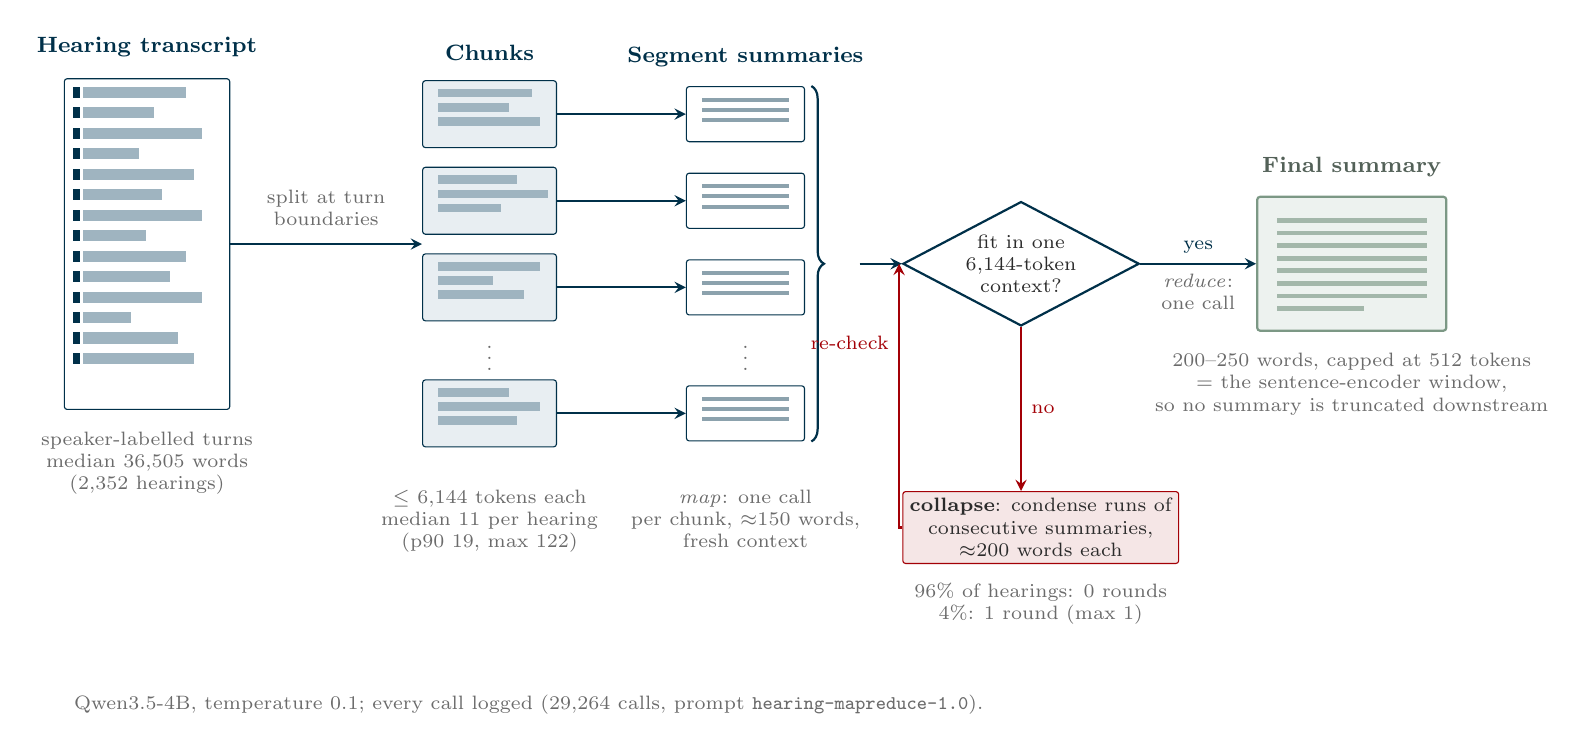
\begin{tikzpicture}[
  font=\footnotesize,
  every node/.style={text=ink},
  stage/.style={font=\footnotesize\bfseries, text=navy},
  note/.style={font=\scriptsize, text=ink!70},
  flow/.style={-{stealth}, navy, thick},
  chunkbox/.style={draw=navy, fill=navylight, rounded corners=1pt,
                   minimum width=17mm, minimum height=8.5mm, inner sep=1.5pt},
  card/.style={draw=navy, fill=white, rounded corners=1pt,
               minimum width=15mm, minimum height=7mm, inner sep=1.5pt},
]

% ---------------------------------------------------------------- transcript
% A tall document with speaker-turn stripes of varying length.
\node[draw=navy, fill=white, minimum width=21mm, minimum height=42mm,
      rounded corners=1pt] (doc) at (0,0) {};
\foreach \y/\w in {17/13, 14.4/9, 11.8/15, 9.2/7, 6.6/14, 4/10, 1.4/15,
                   -1.2/8, -3.8/13, -6.4/11, -9/15, -11.6/6, -14.2/12, -16.8/14}{
  \fill[navymid] ($(doc.north west)+(2.5mm,-19.5mm+\y mm)$) rectangle
                 ++(\w mm,1.4mm);
  \fill[navy]    ($(doc.north west)+(1.2mm,-19.5mm+\y mm)$) rectangle
                 ++(0.9mm,1.4mm);
}
\node[stage, anchor=south] at ($(doc.north)+(0,1.5mm)$) {Hearing transcript};
\node[note, anchor=north, align=center] at ($(doc.south)+(0,-1.5mm)$)
  {speaker-labelled turns\\median 36{,}505 words\\(2{,}352 hearings)};

% ---------------------------------------------------------------- chunking
\node[chunkbox] (c1) at (4.35,1.65) {};
\node[chunkbox] (c2) at (4.35,0.55) {};
\node[chunkbox] (c3) at (4.35,-0.55) {};
\node[note] (cdots) at (4.35,-1.35) {$\vdots$};
\node[chunkbox] (c4) at (4.35,-2.15) {};
\foreach \b/\rows in {c1/{2.2/12,4.0/9,5.8/13}, c2/{2.2/10,4.0/14,5.8/8},
                      c3/{2.2/13,4.0/7,5.8/11}, c4/{2.2/9,4.0/13,5.8/10}}{
  \foreach \y/\w in \rows {
    \fill[navymid] ($(\b.north west)+(2mm,-\y mm)$) rectangle ++(\w mm,1.1mm);
  }
}
\node[stage, anchor=south] at ($(c1.north)+(0,1.2mm)$) {Chunks};
\draw[flow] (doc.east) -- (c1.west|-doc.east)
  node[midway, above, note, align=center, yshift=1mm]
  {split at turn\\boundaries};
\node[note, anchor=north, align=center] at (4.35,-3.0)
  {$\le$ 6{,}144 tokens each\\median 11 per hearing\\(p90 19, max 122)};

% ---------------------------------------------------------------- map
\node[card] (s1) at (7.6,1.65) {};
\node[card] (s2) at (7.6,0.55) {};
\node[card] (s3) at (7.6,-0.55) {};
\node[note] (sdots) at (7.6,-1.35) {$\vdots$};
\node[card] (s4) at (7.6,-2.15) {};
\foreach \b in {s1,s2,s3,s4}{
  \foreach \y in {1.6, 0.3, -1.0}{
    \fill[navy!45] ($(\b.center)+(-5.5mm,\y mm)$) rectangle ++(11mm,0.5mm);
  }
}
\node[stage, anchor=south, align=center] at ($(s1.north)+(0,1.2mm)$)
  {Segment summaries};
\foreach \a/\b in {c1/s1, c2/s2, c3/s3, c4/s4}{
  \draw[flow] (\a.east) -- (\b.west);
}
\node[note, anchor=north, align=center] at (7.6,-3.0)
  {\emph{map}: one call\\per chunk, $\approx$150 words,\\fresh context};

% ---------------------------------------------------------------- budget check
\node[draw=navy, thick, diamond, aspect=1.9, fill=white, inner sep=1pt,
      align=center, font=\scriptsize] (fit) at (11.1,-0.25)
  {fit in one\\6{,}144-token\\context?};
\draw[decorate, decoration={brace, amplitude=1.6mm}, navy, thick]
  ($(s1.north east)+(0.8mm,0)$) -- ($(s4.south east)+(0.8mm,0)$);
\draw[flow] (9.05,-0.25) -- (fit.west);

% collapse loop (the red, recursive path)
\node[draw=red1, fill=redlight, rounded corners=1pt, align=center,
      font=\scriptsize, inner sep=2.5pt] (col) at (11.35,-3.6)
  {\textbf{collapse}: condense runs of\\consecutive summaries,\\$\approx$200 words each};
\draw[-{stealth}, red1, thick] (fit.south) -- (fit.south|-col.north)
  node[midway, right, font=\scriptsize, text=red1] {no};
\draw[-{stealth}, red1, thick] (col.west) -- (9.55,-3.6) -- (9.55,-0.25)
  node[pos=0.7, left, font=\scriptsize, text=red1] {re-check};
\node[note, anchor=north, align=center] at ($(col.south)+(0,-1.2mm)$)
  {96\% of hearings: 0 rounds\\4\%: 1 round (max 1)};

% ---------------------------------------------------------------- reduce
\node[draw=green1, thick, fill=greenlight, rounded corners=1pt,
      minimum width=24mm, minimum height=17mm] (fin) at (15.3,-0.25) {};
\foreach \y in {5.2, 3.6, 2.0, 0.4, -1.2, -2.8, -4.4}{
  \fill[green1!70] ($(fin.center)+(-9.5mm,\y mm)$) rectangle ++(19mm,0.6mm);
}
\fill[green1!70] ($(fin.center)+(-9.5mm,-6.0mm)$) rectangle ++(11mm,0.6mm);
\node[stage, anchor=south, text=green1!50!ink] at ($(fin.north)+(0,1.2mm)$)
  {Final summary};
\draw[flow] (fit.east) -- (fin.west)
  node[midway, above, font=\scriptsize, text=navy] {yes}
  node[midway, below, note, align=center] {\emph{reduce}:\\one call};
\node[note, anchor=north, align=center] at ($(fin.south)+(0,-1.5mm)$)
  {200--250 words, capped at 512 tokens\\= the sentence-encoder window,\\so no summary is truncated downstream};

% ---------------------------------------------------------------- footer
\node[note, anchor=north west, align=left] at (-1.05,-5.6)
  {Qwen3.5-4B, temperature 0.1; every call logged (29{,}264 calls, prompt \texttt{hearing-mapreduce-1.0}).};

\end{tikzpicture}
\end{document}
